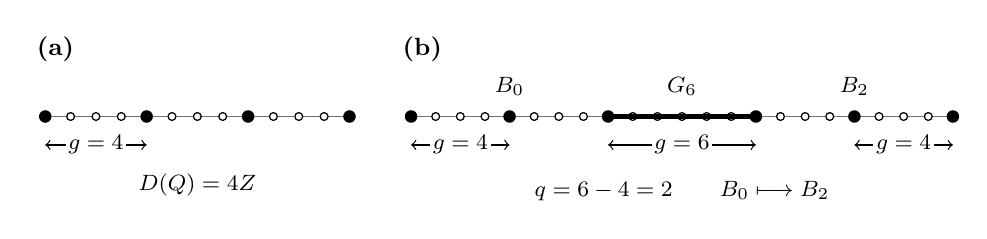
\begin{tikzpicture}[
  x=0.92cm,
  y=0.82cm,
  line cap=round,
  line join=round,
  positive/.style={circle,fill=black,inner sep=1.6pt},
  negative/.style={circle,draw=black,fill=white,inner sep=1.0pt,
    line width=0.45pt},
  bulk/.style={draw=black!55,line width=0.65pt},
  defect/.style={draw=black,line width=1.55pt},
  panel/.style={font=\small\bfseries,anchor=west},
  label/.style={font=\footnotesize,align=center}
]
  % (a) Period-eight reference bulk.
  \node[panel] at (0,2.62) {(a)};
  \draw[bulk] (0.25,1.58)--(4.45,1.58);
  \foreach \i in {0,...,12} {
    \pgfmathtruncatemacro{\r}{mod(\i,4)}
    \ifnum\r=0
      \node[positive] at ({0.25+0.35*\i},1.58) {};
    \else
      \node[negative] at ({0.25+0.35*\i},1.58) {};
    \fi
  }
  \draw[<->,line width=0.45pt]
    (0.25,1.14)--node[label,fill=white,inner sep=1pt]
    {$g=4$} (1.65,1.14);
  \node[label] at (2.35,0.52) {$D(Q)=4\mathbb Z$};

  % (b) Bilateral six-gap phase slip with gaps 4,4,6,4,4.
  \node[panel] at (5.05,2.62) {(b)};
  \draw[bulk] (5.30,1.58)--(12.78,1.58);
  \foreach \i in {0,...,22} {
    \node[negative] at ({5.30+0.34*\i},1.58) {};
  }
  \foreach \i in {0,4,8,14,18,22} {
    \node[positive] at ({5.30+0.34*\i},1.58) {};
  }
  \draw[defect] (8.02,1.58)--(10.06,1.58);
  \node[label] at (6.66,2.05) {$B_0$};
  \node[label] at (9.04,2.05) {$G_6$};
  \node[label] at (11.42,2.05) {$B_2$};
  \draw[<->,line width=0.45pt]
    (5.30,1.14)--node[label,fill=white,inner sep=1pt]
    {$g=4$} (6.66,1.14);
  \draw[<->,line width=0.45pt]
    (8.02,1.14)--node[label,fill=white,inner sep=1pt]
    {$g=6$} (10.06,1.14);
  \draw[<->,line width=0.45pt]
    (11.42,1.14)--node[label,fill=white,inner sep=1pt]
    {$g=4$} (12.78,1.14);
  \node[label] at (9.04,0.42)
    {$q=6-4=2$\qquad $B_0\longmapsto B_2$};
\end{tikzpicture}
